\documentclass[a4paper,10pt]{article}
\usepackage[utf8]{inputenc}
\usepackage{polski}
\usepackage[T1]{fontenc}
\usepackage{lmodern}
\usepackage[most]{tcolorbox}
\usepackage{inconsolata}
\usepackage{listings}
\usepackage{caption}
\usepackage[margin=0.5in]{geometry}

%opening
\title{Teoria Współbieżności - ćwiczenie}
\author{Mateusz Szarek}
\date{}

\begin{document}

\maketitle

\section{Zadanie}
Proszę zaimplementować przy użyciu mechanizmów Executor i Future program wykonujący obliczanie zbioru Mandelbrota w puli wątkówk. Jako podstawę implementacji proszę wykorzystać kod w Javie. Uwaga: pojedyncze zadanie powinno obliczać podzbiór całego zbioru (np. kilka wierszy). Problem proszę podzielić tak, żeby liczba zadań była rzędu 10 x liczba wątków.\\
Proszę przetestować szybkość działania programu w zależności od implementacji Executora i jego parametrów (np. liczba wątków w puli). Czas obliczeń można zwiększać manipulując parametrami problemu.

\section{Wyniki}

\subsection*{Parametry}

W celu wykonania ćwiczenia, przyjąłem następujące wartości: wysokość (600), szerokość (800), grid (200x200).

\subsection*{Wykonanie}

Pomiary wykonywałem na kodzie wykonanym własnoręcznie, testuję czas dla następującej ilości wątków:
\begin{enumerate}
 \item SingleThreadedExecutor - 1 rdzeń
 \item MultiThreadedExecutor - 1 rdzeń
 \item MultiThreadedExecutor- 2 rdzenie
 \item MultiThreadedExecutor - 3 rdzenie
 \item MultiThreadedExecutor - 4 rdzenie
 \item MultiThreadedExecutor - 8 rdzeni
\end{enumerate}
Wszystkie pomiary przedstawiłem na wykresach. Na osi OX znajduje się ilość wątków biorących udział w pomiarach, na osi OY znajduje się czas wykonania. Dla każdej ilości wątków wykonałem po 10 pomiarów. Dane posiadam na lokalnym dysku.


\subsection*{Wyniki}

\subsection{MAX\_ITER = 5000}

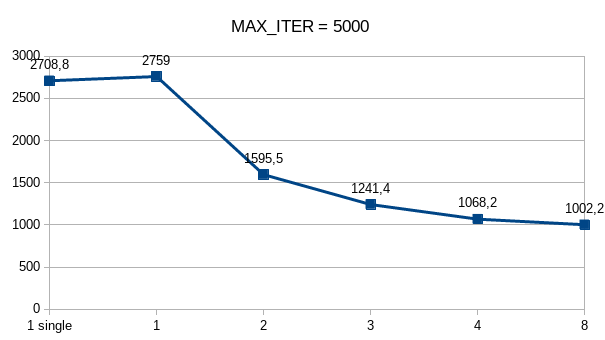
\includegraphics[width=\textwidth]{1.png}

\vspace*{20mm}

\subsection{MAX\_ITER = 10000}

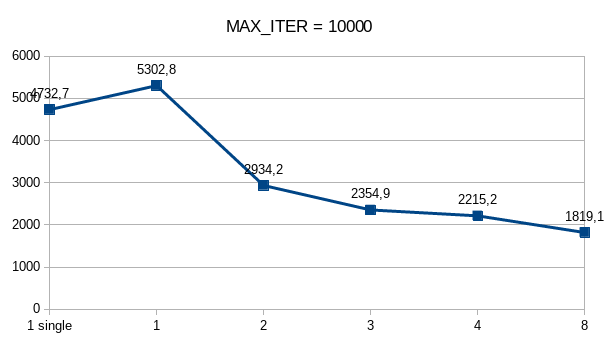
\includegraphics[width=\textwidth]{2.png}

\subsection{MAX\_ITER = 15000}

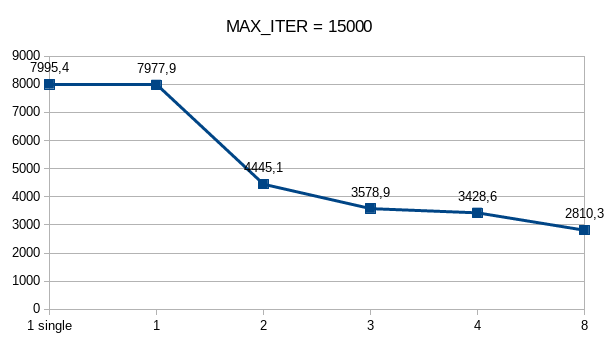
\includegraphics[width=\textwidth]{3.png}
\vspace*{10mm}\\
\section*{Podsumowanie}
Jak widzimy, im więcej pracy do wykonania tym większy zysk otrzymujemy na Współbieżności. Niestety dla mniejszej ilości rdzeni, a także często dla naszego prywatnego komputera, aplikacje współbieżne nie mają sensu być instalowane.
\end{document}
